% \documentclass[handout,aspectratio=169,11pt]{beamer}
\documentclass[aspectratio=169,11pt]{beamer}

\usepackage[T1]{fontenc}
\usepackage[utf8]{inputenc}
\usepackage[english]{babel}
\usepackage{csquotes}
\usepackage{lmodern}
\usepackage{amsmath,amssymb}
\usepackage{cancel}
\usepackage{tikz}
\usepackage{fontawesome5}
\usepackage{verbatim}
\usepackage{pgfplots}
\usepackage{booktabs}
\pgfplotsset{compat=1.18}
\usepackage{subcaption}
\usetikzlibrary{decorations.pathreplacing, positioning}
\usepackage{listings}
\usepackage{hyperref}
\usepackage[backend=biber,style=authoryear]{biblatex}
\addbibresource{references.bib}

\usetheme{Warsaw}
\usecolortheme{wolverine}
\usefonttheme{serif}
\useinnertheme{circles}
\useoutertheme{shadow}

\hypersetup{
  colorlinks=true,
  linkcolor=black,
  filecolor=cyan,
  citecolor=gray,
  urlcolor=magenta,
  pdftitle={A Quick Intro to Python Programming},
}

\setbeamertemplate{footline}[frame number]
\setbeamertemplate{note page}[plain]
\setbeamertemplate{navigation symbols}{}
\setbeamercovered{transparent}
\setbeamertemplate{headline}{}

\lstdefinestyle{pythoncompact}{
  language=Python,
  basicstyle=\ttfamily\footnotesize,
  keywordstyle=\color{blue!70!black}\bfseries,
  commentstyle=\color{green!50!black}\itshape,
  stringstyle=\color{red!70!black},
  showstringspaces=false,
  breaklines=true,
  tabsize=2,
  columns=fullflexible,
}

\lstdefinestyle{pythonTiny}{
  language=Python,
  basicstyle=\ttfamily\scriptsize,
  keywordstyle=\color{blue!70!black}\bfseries,
  commentstyle=\color{green!50!black}\itshape,
  stringstyle=\color{red!70!black},
  showstringspaces=false,
  breaklines=true,
  tabsize=2,
  columns=fullflexible,
}

\lstdefinestyle{terminal}{
  basicstyle=\ttfamily\footnotesize,
  showstringspaces=false,
  breaklines=true,
  columns=fullflexible,
}


\title{A Quick Intro to Python Programming}
\subtitle{Scientific computing with a kinematics example}
\author{Manuel A. Diaz}
\institute{InspiraSTEM Internship}
\date{\today}
\titlegraphic{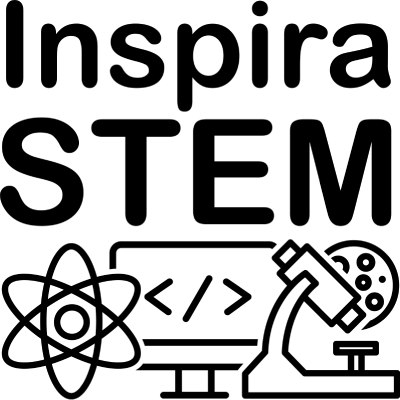
\includegraphics[height=1.35cm]{figures/InspiraSTEM_logo.png}}

\AtBeginSection[]{
  \begin{frame}{Outline}
    \tableofcontents[currentsection]
  \end{frame}
}

%%%%%%%%%%%%%%%%%%%
\begin{document}
%%%%%%%%%%%%%%%%%%%

\begin{frame}
  \titlepage
\end{frame}

\begin{frame}{Outline}
  \tableofcontents
\end{frame}

\begin{frame}{This is a very quick intro to Python programming}
  \begin{itemize}
    \item variables for numbers, lists, and arrays
    \item while loops and for loops
    \item functions
    \item if tests
    \item plotting
    \item files
    \item classes
  \end{itemize}
  \vspace{1em}
  Method: show program code through math examples
\end{frame}

\section{Variables, loops, lists, and arrays}

\begin{frame}[fragile]{Do you have access to Python?}
  For this course we use \href{https://docs.astral.sh/uv/}{uv} to install Python and packages.

  \begin{enumerate}
    \item Install \texttt{uv}
    \item At the project root (folder with \texttt{pyproject.toml}):
  \end{enumerate}
\begin{lstlisting}[style=terminal]
uv sync
cd python_intro
uv run python distance.py
\end{lstlisting}
  \texttt{uv run} uses the project environment; no manual \texttt{venv} activation needed.
\end{frame}

\begin{frame}{Mathematical example}
  Most examples will involve this formula:
  \begin{equation}
    s = v_0 t + \frac{1}{2} a t^2
  \end{equation}
  We may view $s$ as a function of $t$: $s(t)$, and also include the
  parameters in the notation: $s(t;v_0,a)$.
\end{frame}

\begin{frame}[fragile]{A program for evaluating a formula}
  \textbf{Task:} Compute $s$ for $t=0.5$, $v_0=2$, and $a=0.2$.

  \textbf{Python code} (\texttt{python\_intro/distance.py}):
\lstinputlisting[style=pythoncompact,firstline=6]{code/distance.py}
\end{frame}

\begin{frame}[fragile]{Execution}
\begin{lstlisting}[style=terminal]
Terminal> uv run python distance.py
1.025
s=1.025
s        =       1.025
\end{lstlisting}
\end{frame}

\begin{frame}[fragile]{Assignment statements assign a name to an object}
\begin{lstlisting}[style=pythoncompact]
t = 0.5                   # real number makes float object
v0 = 2                    # integer makes int object
a = 0.2                   # float object
s = v0*t + 0.5*a*t**2     # float object
\end{lstlisting}
  Rule:
  \begin{itemize}
    \item evaluate right-hand side; it results in an \emph{object}
    \item left-hand side is a name for that object
  \end{itemize}
\end{frame}

\begin{frame}[fragile]{Formatted output with text and numbers}
  \begin{itemize}
    \item Task: write out text with a number (3 decimals): \texttt{s=1.025}
    \item Method: f-strings (modern Python)
  \end{itemize}
\begin{lstlisting}[style=pythoncompact]
print(f's={s:g}')       # g: compact notation
print(f's={s:.2f}')     # f: decimal notation, 2 decimals
\end{lstlisting}
  Older alternatives (still valid):
\begin{lstlisting}[style=pythoncompact]
print('s=%g' % s)
print('s={s:.2f}'.format(s=s))
\end{lstlisting}
\end{frame}

\begin{frame}[fragile]{Programming with a while loop}
  \begin{itemize}
    \item Task: write out a table of $t$ and $s(t)$ values (two columns),
          for $t\in [0,2]$ in steps of $0.1$
    \item Method: while loop
  \end{itemize}
\lstinputlisting[style=pythonTiny,firstline=7]{code/while.py}
\end{frame}

\begin{frame}[fragile]{Output of the previous program}
\begin{lstlisting}[style=terminal]
Terminal> uv run python while.py
0 0.0
0.1 0.201
0.2 0.404
0.3 0.609
0.4 0.816
0.5 1.025
...
1.8 3.924
1.9 4.161
\end{lstlisting}
\end{frame}

\begin{frame}[fragile]{Structure of a while loop}
\begin{lstlisting}[style=pythoncompact]
while condition:
    <indented statement>
    <indented statement>
    <indented statement>
\end{lstlisting}
  Note:
  \begin{itemize}
    \item the colon in the first line
    \item all statements in the loop \emph{must be indented}\\
          (no braces as in C, C++, Java, \ldots)
    \item \texttt{condition} is a boolean expression (e.g., \texttt{t <= 2})
  \end{itemize}
\end{frame}

\begin{frame}[fragile]{Closer look at the output}
\begin{lstlisting}[style=terminal]
Terminal> uv run python while.py
0 0.0
0.1 0.201
...
1.8 3.924
1.9 4.161
\end{lstlisting}
  The last line contains $1.9$, but the while loop should run also when
  $t=2$ since the test is \texttt{t <= 2}. Why is this test \texttt{False}?
\end{frame}

\begin{frame}[fragile]{Examine the program (Python Tutor idea)}
  Step through a smaller loop and examine variables
  (\href{https://pythontutor.com/visualize.html\#mode=edit}{Python Tutor}):
\begin{lstlisting}[style=pythoncompact]
a = 0
da = 0.4
while a <= 1.2:
    print(a)
    a = a + da
\end{lstlisting}
\end{frame}

\begin{frame}[fragile]{Round-off errors!}
  Why is \texttt{a <= 1.2} false when \texttt{a} ``is'' $1.2$?
\begin{lstlisting}[style=pythoncompact]
a = 0
da = 0.4
while a <= 1.2:
    print(a)
    a = a + da
    print(f'da={da:.16E}\na={a:.16E}')
    print(f'a <= 1.2: {a <= 1.2}')
\end{lstlisting}
  \begin{alertblock}{Key point}
    Small round-off error in \texttt{da} makes
    \texttt{a = 1.2000000000000002}
  \end{alertblock}
\end{frame}

\begin{frame}[fragile]{Never \texttt{a == b} for real numbers}
  Always use a tolerance!
\begin{lstlisting}[style=pythoncompact]
a = 1.2
b = 0.4 + 0.4 + 0.4
boolean_condition1 = a == b              # may be False

# This is the way to do it
tol = 1E-14
boolean_condition2 = abs(a - b) < tol    # True
\end{lstlisting}
\end{frame}

\begin{frame}[fragile]{A list collects several objects in a sequence}
  A list of numbers:
\begin{lstlisting}[style=pythoncompact]
L = [-1, 1, 8.0]
\end{lstlisting}
  A list can contain any type of objects:
\begin{lstlisting}[style=pythoncompact]
L = ['mydata.txt', 3.14, 10]   # string, float, int
\end{lstlisting}
\end{frame}

\begin{frame}[fragile]{Basic list operations}
\begin{lstlisting}[style=pythonTiny]
>>> L = ['mydata.txt', 3.14, 10]
>>> print(L[0])    # first element (index 0)
mydata.txt
>>> print(L[1])    # second element (index 1)
3.14
>>> del L[0]       # delete the first element
>>> print(L)
[3.14, 10]
>>> print(len(L))  # length of L
2
>>> L.append(-1)   # add -1 at the end
>>> print(L)
[3.14, 10, -1]
\end{lstlisting}
\end{frame}

\begin{frame}[fragile]{Store our table in two lists}
\lstinputlisting[style=pythonTiny,firstline=7]{code/while_list.py}
\end{frame}

\begin{frame}[fragile]{For loops}
  A for loop visits elements in a list, one by one:
\begin{lstlisting}[style=pythoncompact]
>>> L = [1, 4, 8, 9]
>>> for e in L:
...     print(e)
...
1
4
8
9
\end{lstlisting}
\end{frame}

\begin{frame}[fragile]{For-loop demo (Python Tutor style)}
\begin{lstlisting}[style=pythoncompact]
list1 = [0, 0.1, 0.2]
list2 = []
for element in list1:
    p = element + 2
    list2.append(p)
print(list2)
\end{lstlisting}
\end{frame}

\begin{frame}[fragile]{Integer counter over list/array indices}
\begin{lstlisting}[style=pythoncompact]
somelist = ['file1.dat', 22, -1.5]

for i in range(len(somelist)):
    # access list element through index
    print(somelist[i])
\end{lstlisting}
  Note:
  \begin{itemize}
    \item \texttt{range} returns a sequence of integers
    \item \texttt{range(a, b, s)} gives \texttt{a, a+s, \ldots} up to
          \emph{but not including} $b$
    \item \texttt{range(b)} implies $a=0$ and $s=1$
    \item \texttt{range(len(somelist))} gives $0,1,2$
  \end{itemize}
\end{frame}

\begin{frame}[fragile]{Replace our while loop by a for loop}
\lstinputlisting[style=pythonTiny,firstline=7]{code/for_list.py}
\end{frame}

\begin{frame}[fragile]{Traversal of multiple lists with \texttt{zip}}
\begin{lstlisting}[style=pythoncompact]
for e1, e2, e3, ... in zip(list1, list2, list3, ...):
\end{lstlisting}
  Alternative: loop over a common index
\begin{lstlisting}[style=pythoncompact]
for i in range(len(list1)):
    e1 = list1[i]
    e2 = list2[i]
    e3 = list3[i]
\end{lstlisting}
\end{frame}

\begin{frame}{Arrays are efficient lists of numbers}
  \begin{itemize}
    \item Lists collect objects in a single variable
    \item Lists are flexible (can grow, can contain ``anything'')
    \item Array: computationally efficient list of numbers
    \item Arrays have fixed length and one numeric type
    \item Arrays require the \texttt{numpy} module
  \end{itemize}
\end{frame}

\begin{frame}[fragile]{Examples on using arrays}
\begin{lstlisting}[style=pythonTiny]
>>> import numpy
>>> L = [1, 4, 10.0]    # List of numbers
>>> a = numpy.array(L)  # Convert to array
>>> print(a)
[ 1.  4. 10.]
>>> print(a[1])         # indexing
4.0
>>> print(a[0:2])       # slice (index 2 not included!)
[1. 4.]
>>> print(a.dtype)      # data type of an element
float64
>>> b = 2*a + 1         # arithmetics on arrays
>>> print(b)
[ 3.  9. 21.]
\end{lstlisting}
\end{frame}

\begin{frame}[fragile]{\texttt{numpy} functions create entire arrays}
  Apply $\ln$ to all elements in array \texttt{a}:
\begin{lstlisting}[style=pythoncompact]
>>> c = numpy.log(a)
>>> print(c)
[0.         1.38629436 2.30258509]
\end{lstlisting}
  Create $n+1$ uniformly spaced coordinates in $[a,b]$:
\begin{lstlisting}[style=pythoncompact]
t = numpy.linspace(a, b, n+1)
\end{lstlisting}
  Array of length $n$ filled with zeros:
\begin{lstlisting}[style=pythoncompact]
t = numpy.zeros(n)
s = numpy.zeros_like(t)  # zeros with t's size and dtype
\end{lstlisting}
\end{frame}

\begin{frame}[fragile]{Let's use arrays in our previous program}
\lstinputlisting[style=pythonTiny,firstline=7]{code/for_array.py}
  Note: no explicit loop for computing \texttt{s\_values}!
\end{frame}

\begin{frame}[fragile]{Standard math functions: the \texttt{math} module}
\begin{lstlisting}[style=pythoncompact]
>>> import math
>>> print(math.sin(math.pi))
1.2246467991473532e-16         # approximate value
\end{lstlisting}
  Get rid of the \texttt{math} prefix:
\begin{lstlisting}[style=pythoncompact]
from math import sin, pi
print(sin(pi))

from math import *   # import everything
print(sin(pi), log(e), tanh(0.5))
\end{lstlisting}
\end{frame}

\begin{frame}[fragile]{Use \texttt{numpy} for math on arrays}
  Matlab-style:
\begin{lstlisting}[style=pythoncompact]
from numpy import *
x = linspace(0, 1, 101)
y = exp(-x)*sin(pi*x)
\end{lstlisting}
  Preferred style:
\begin{lstlisting}[style=pythoncompact]
import numpy as np
x = np.linspace(0, 1, 101)
y = np.exp(-x)*np.sin(np.pi*x)
\end{lstlisting}
\end{frame}

\begin{frame}[fragile]{Our convention: \texttt{np} prefix, clean formulas}
\begin{lstlisting}[style=pythoncompact]
import numpy as np
x = np.linspace(0, 1, 101)

from numpy import sin, exp, pi
y = exp(-x)*sin(pi*x)
\end{lstlisting}
\end{frame}

\begin{frame}[fragile]{Array assignment gives a view (no copy!)}
  Consider array assignment \texttt{b = a}:
\begin{lstlisting}[style=pythoncompact]
a = np.linspace(1, 5, 5)
b = a
\end{lstlisting}
  Here, \texttt{b} is a \emph{view} (pointer) to the data of \texttt{a} ---
  no copying of data!
\begin{lstlisting}[style=pythonTiny]
>>> a
array([1., 2., 3., 4., 5.])
>>> b[0] = 5                          # changes a[0] to 5
>>> a
array([5., 2., 3., 4., 5.])
>>> a[1] = 9                          # changes b[1] to 9
>>> b
array([5., 9., 3., 4., 5.])
\end{lstlisting}
\end{frame}

\begin{frame}[fragile]{Copying array data: the \texttt{copy} method}
\begin{lstlisting}[style=pythonTiny]
>>> c = a.copy()       # copy all elements to new array c
>>> c[0] = 6           # a is not changed
>>> a
array([1., 2., 3., 4., 5.])
>>> c
array([6., 2., 3., 4., 5.])
\end{lstlisting}
\end{frame}

\begin{frame}{Construction of tridiagonal and sparse matrices}
  \begin{itemize}
    \item SciPy offers
          \href{https://docs.scipy.org/doc/scipy/reference/sparse.html}{scipy.sparse}
    \item Build sparse matrices from diagonals with \texttt{diags}
          (or the newer \texttt{diags\_array})
    \item Super-/sub-diagonals are shorter than the main diagonal
    \item Scalar broadcasting is supported (specify \texttt{shape})
  \end{itemize}
\end{frame}

\begin{frame}[fragile]{Tridiagonal matrix with \texttt{diags}}
\begin{lstlisting}[style=pythonTiny]
>>> import numpy as np
>>> import scipy.sparse
>>> N = 6
>>> diagonals = [
...     -np.linspace(1, N, N)[:-1],
...     -2*np.ones(N),
...     np.linspace(1, N, N)[1:],
... ]
>>> A = scipy.sparse.diags(diagonals, [-1, 0, 1], format='csc')
>>> A.toarray()
[[-2.  2.  0.  0.  0.  0.]
 [-1. -2.  3.  0.  0.  0.]
 [ 0. -2. -2.  4.  0.  0.]
 [ 0.  0. -3. -2.  5.  0.]
 [ 0.  0.  0. -4. -2.  6.]
 [ 0.  0.  0.  0. -5. -2.]]
\end{lstlisting}
\end{frame}

\begin{frame}[fragile]{Scalar broadcasting with \texttt{diags}}
\begin{lstlisting}[style=pythonTiny]
>>> B = scipy.sparse.diags(
...     [1, 2, 3], [-2, 0, 1], shape=(6, 6), format='csc')
>>> B.toarray()
[[2. 3. 0. 0. 0. 0.]
 [0. 2. 3. 0. 0. 0.]
 [1. 0. 2. 3. 0. 0.]
 [0. 1. 0. 2. 3. 0.]
 [0. 0. 1. 0. 2. 3.]
 [0. 0. 0. 1. 0. 2.]]
\end{lstlisting}
\end{frame}

\begin{frame}[fragile]{Legacy note: \texttt{spdiags}}
  Older code may use \texttt{spdiags}: all diagonals must have length $N$;
  unused entries sit at the start of super-diagonals and the end of
  sub-diagonals.
\begin{lstlisting}[style=pythonTiny]
>>> diagonals = np.zeros((3, N))
>>> diagonals[0, :] = np.linspace(-1, -N, N)
>>> diagonals[1, :] = -2
>>> diagonals[2, :] = np.linspace(1, N, N)
>>> A = scipy.sparse.spdiags(
...     diagonals, [-1, 0, 1], N, N, format='csc')
\end{lstlisting}
  Prefer \texttt{diags} / \texttt{diags\_array} in new code.
\end{frame}

\begin{frame}[fragile]{Solving a tridiagonal system}
  Solve $Ax=b$: choose $x$, compute $b=Ax$, solve, check.
\begin{lstlisting}[style=pythonTiny]
>>> x = np.linspace(-1, 1, N)
>>> b = A @ x                    # sparse matrix-vector product
>>> import scipy.sparse.linalg
>>> x = scipy.sparse.linalg.spsolve(A, b)
>>> print(x)
[-1.  -0.6 -0.2  0.2  0.6  1. ]
\end{lstlisting}
\end{frame}

\begin{frame}[fragile]{Check against dense matrix computations}
\begin{lstlisting}[style=pythonTiny]
>>> A_d = A.toarray()
>>> b = A_d @ x                  # dense product
>>> x = np.linalg.solve(A_d, b)
>>> print(x)
[-1.  -0.6 -0.2  0.2  0.6  1. ]
\end{lstlisting}
  See also \texttt{scipy\_intro/tridiagonal.py} in this repository.
\end{frame}

\begin{frame}[fragile]{Plotting}
  Plotting is done with \texttt{matplotlib}:
\lstinputlisting[style=pythonTiny,firstline=7]{code/plot1.py}
\end{frame}

\begin{frame}[fragile]{Plotting of multiple curves}
  Core idea (see \texttt{python\_intro/plot2.py}):
\begin{lstlisting}[style=pythonTiny]
v0, a0, a1, n = 0.2, 2, 3, 21
t = np.linspace(0, 2, n + 1)
s0 = v0 * t + 0.5 * a0 * t**2
s1 = v0 * t + 0.5 * a1 * t**2
plt.plot(t, s0, 'r-', t, s1, 'bo')
plt.xlabel('t [s]'); plt.ylabel('s [m]')
plt.legend([rf'$s(t; v_0={v0}, a={a0})$',
            rf'$s(t; v_0={v0}, a={a1})$'])
\end{lstlisting}
\end{frame}

\section{Functions and branching}

\begin{frame}[fragile]{Functions}
  \begin{itemize}
    \item $s(t)=v_0t + \frac{1}{2}at^2$ is a mathematical function
    \item Can implement $s(t)$ as a Python function \texttt{s(t)}
  \end{itemize}
\begin{lstlisting}[style=pythoncompact]
def s(t):
    return v0*t + 0.5*a*t**2

v0 = 0.2
a = 4
value = s(3)   # Call the function
\end{lstlisting}
\end{frame}

\begin{frame}{Function notes}
  \begin{itemize}
    \item functions start with the keyword \texttt{def}
    \item statements belonging to the function must be indented
    \item function input is represented by arguments
          (comma-separated if more than one)
    \item function output is returned to the calling code
    \item \texttt{v0} and \texttt{a} above are \emph{global variables},
          which must be initialized before \texttt{s(t)} is called
  \end{itemize}
\end{frame}

\begin{frame}[fragile]{Functions can have multiple arguments}
  \texttt{v0} and \texttt{a} as function arguments instead of globals:
\begin{lstlisting}[style=pythoncompact]
def s(t, v0, a):
    return v0*t + 0.5*a*t**2

value = s(3, 0.2, 4)   # Call the function

# More readable call
value = s(t=3, v0=0.2, a=4)
\end{lstlisting}
\end{frame}

\begin{frame}[fragile]{Keyword arguments (default values)}
\begin{lstlisting}[style=pythoncompact]
def s(t, v0=1, a=1):
    return v0*t + 0.5*a*t**2

value = s(3, 0.2, 4)         # specify new v0 and a
value = s(3)                 # rely on v0=1 and a=1
value = s(3, a=2)            # rely on v0=1
value = s(3, v0=2)           # rely on a=1
value = s(t=3, v0=2, a=2)    # specify everything
value = s(a=2, t=3, v0=2)    # any keyword order
\end{lstlisting}
\end{frame}

\begin{frame}{Positional vs keyword arguments}
  \begin{itemize}
    \item Arguments without the argument name are \emph{positional}
    \item Positional arguments must always be listed before keyword
          arguments in the definition and in any call
    \item The sequence of keyword arguments can be arbitrary
  \end{itemize}
\end{frame}

\begin{frame}[fragile]{Vectorization speeds up the code}
  Scalar code (one number at a time):
\begin{lstlisting}[style=pythoncompact]
def s(t, v0, a):
    return v0*t + 0.5*a*t**2

for i in range(len(t_values)):
    s_values[i] = s(t_values[i], v0, a)
\end{lstlisting}
  Vectorized code: apply \texttt{s} to the entire array
\begin{lstlisting}[style=pythoncompact]
s_values = s(t_values, v0, a)
\end{lstlisting}
\end{frame}

\begin{frame}{How can vectorization work?}
  Expression \texttt{v0*t + 0.5*a*t**2} with array \texttt{t}:
  \begin{itemize}
    \item \texttt{r1 = v0*t} (scalar times array)
    \item \texttt{r2 = t**2} (square each element)
    \item \texttt{r3 = 0.5*a*r2} (scalar times array)
    \item \texttt{r1 + r3} (add each element)
  \end{itemize}
\end{frame}

\begin{frame}[fragile]{Scalar functions often work for arrays too}
  True if computations involve arithmetic and math functions:
\begin{lstlisting}[style=pythoncompact]
from math import exp, sin

def f(x):
    return 2*x + x**2*exp(-x)*sin(x)

v = f(4)  # works with scalar x

from numpy import exp, sin, linspace
x = linspace(0, 4, 100001)
v = f(x)  # now works with array x
\end{lstlisting}
\end{frame}

\begin{frame}[fragile]{Functions can return multiple values}
  Return $s(t)=v_0t+\frac{1}{2}at^2$ and $s'(t)=v_0 + at$:
\begin{lstlisting}[style=pythoncompact]
def movement(t, v0, a):
    s = v0*t + 0.5*a*t**2
    v = v0 + a*t
    return s, v

s_value, v_value = movement(t=0.2, v0=2, a=4)
\end{lstlisting}
\end{frame}

\begin{frame}[fragile]{Multiple return values are a tuple}
  \texttt{return s, v} returns a \emph{tuple} ($\approx$ immutable list):
\begin{lstlisting}[style=pythonTiny]
>>> def f(x):
...     return x+1, x+2, x+3
...
>>> r = f(3)
>>> print(r)
(4, 5, 6)
>>> type(r)
<class 'tuple'>
>>> print(r[1])
5
\end{lstlisting}
  Tuples are constant lists (cannot be changed).
\end{frame}

\begin{frame}{A more general formula (part I)}
  Equations from basic kinematics:
  \begin{align*}
    v = \frac{ds}{dt},\quad s(0)=s_0\\
    a = \frac{dv}{dt},\quad v(0)=v_0
  \end{align*}
  Integrate to find $v(t)$:
  \[
    \int_0^t a(t)\,dt = \int_0^t \frac{dv}{dt}\,dt
  \]
  which gives
  \[
    v(t) = v_0 + \int_0^t a(t)\,dt
  \]
\end{frame}

\begin{frame}{A more general formula (part II)}
  Integrate again over $[0,t]$ to find $s(t)$:
  \[
    s(t) = s_0 + v_0 t + \int_0^t\left( \int_0^\tau a(\xi)\,d\xi \right) d\tau
  \]
  Example: $a(t)=a_0$ for $t\in[0,t_1]$, then $a(t)=0$ for $t>t_1$:
  \[
  s(t) =
  \begin{cases}
  s_0 + v_0 t + \tfrac12 a_0 t^2, & t\leq t_1\\[0.5em]
  s_0 + v_0 t_1 + \tfrac12 a_0 t_1^2 + a_0 t_1(t-t_1), & t> t_1
  \end{cases}
  \]
  Need an \emph{if} test to implement this!
\end{frame}

\begin{frame}[fragile]{Basic if-else tests}
\begin{lstlisting}[style=pythoncompact]
if condition:
    <statements when condition is True>
else:
    <statements when condition is False>
\end{lstlisting}
  Here, \texttt{condition} is a boolean expression with value
  \texttt{True} or \texttt{False}.
\begin{lstlisting}[style=pythoncompact]
if t <= t1:
    s = v0*t + 0.5*a0*t**2
else:
    s = v0*t + 0.5*a0*t1**2 + a0*t1*(t-t1)
\end{lstlisting}
\end{frame}

\begin{frame}[fragile]{Multi-branch if tests}
\begin{lstlisting}[style=pythonTiny]
if condition1:
    <statements when condition1 is True>
elif condition2:
    <when condition1 is False and condition2 is True>
elif condition3:
    <when 1 and 2 are False and condition3 is True>
else:
    <when condition1/2/3 all are False>
\end{lstlisting}
  Just if, no else:
\begin{lstlisting}[style=pythoncompact]
if condition:
    <statements when condition is True>
\end{lstlisting}
\end{frame}

\begin{frame}[fragile]{Piecewise function with if}
\begin{lstlisting}[style=pythonTiny]
def s_func(t, v0, a0, t1):
    if t <= t1:
        s = v0 * t + 0.5 * a0 * t**2
    else:
        s = (v0 * t + 0.5 * a0 * t1**2
             + a0 * t1 * (t - t1))
    return s
\end{lstlisting}
  Full demo: \texttt{python\_intro/plot3.py}
\end{frame}

\begin{frame}[fragile]{If + arrays: does not work}
\begin{lstlisting}[style=pythonTiny]
>>> def f(x):
...     return x if x < 1 else 2*x
...
>>> import numpy as np
>>> x = np.linspace(0, 2, 5)
>>> f(x)
ValueError: The truth value of an array with more than one
element is ambiguous. Use a.any() or a.all()
\end{lstlisting}
  Problem: \texttt{x < 1} evaluates to a boolean array, not a single boolean.
\end{frame}

\begin{frame}[fragile]{Remedy 1: call with scalar arguments}
\begin{lstlisting}[style=pythonTiny]
n = 201
t1 = 1.5
v0 = 0.2
a0 = 20
t = np.linspace(0, 2, n + 1)
s = np.zeros(n + 1)
for i in range(len(t)):
    s[i] = s_func(t=t[i], v0=v0, a0=a0, t1=t1)

plt.plot(t, s, 'b-')
plt.plot([t1, t1], [0, s_func(t=t1, v0=v0, a0=a0, t1=t1)], 'r--')
\end{lstlisting}
\end{frame}

\begin{frame}[fragile]{Remedy 2: vectorize with \texttt{where}}
\begin{lstlisting}[style=pythoncompact]
s = np.where(condition, s1, s2)
\end{lstlisting}
  \begin{itemize}
    \item \texttt{condition}: array of boolean values
    \item \texttt{s[i] = s1[i]} if \texttt{condition[i]} is \texttt{True}
    \item \texttt{s[i] = s2[i]} if \texttt{condition[i]} is \texttt{False}
  \end{itemize}
\begin{lstlisting}[style=pythonTiny]
s = np.where(t <= t1,
             v0*t + 0.5*a0*t**2,
             v0*t + 0.5*a0*t1**2 + a0*t1*(t-t1))
\end{lstlisting}
\end{frame}

\begin{frame}[fragile]{Remedy 3: vectorize with array indexing}
  \begin{itemize}
    \item Let \texttt{b} be a boolean array (e.g.\ \texttt{b = t <= t1})
    \item \texttt{s[b]} selects elements where \texttt{b[i]} is \texttt{True}
    \item Assign: \texttt{s[b] = (expr)[b]}
  \end{itemize}
\begin{lstlisting}[style=pythonTiny]
s = np.zeros_like(t)
s[t <= t1] = (v0*t + 0.5*a0*t**2)[t <= t1]
s[t > t1]  = (v0*t + 0.5*a0*t1**2
              + a0*t1*(t-t1))[t > t1]
\end{lstlisting}
  See also \texttt{python\_intro/plot3\_vec.py}.
\end{frame}

\section{Files}

\begin{frame}[fragile]{File reading}
  Put input data in a text / YAML file (modern approach in this repo):
\begin{lstlisting}[style=terminal]
# input.yaml
v0: 2.0
a: 0.2
dt: 0.1
interval: [0, 2]
\end{lstlisting}
  \begin{alertblock}{Question}
    How can we read this file into variables \texttt{v0}, \texttt{a},
    \texttt{dt}, and \texttt{interval}?
  \end{alertblock}
\end{frame}

\begin{frame}[fragile]{Reading parameters with YAML}
\lstinputlisting[style=pythonTiny,firstline=7,lastline=26]{code/for_file_read_input.py}
\end{frame}

\begin{frame}[fragile]{Classic line parsing: \texttt{variable = value}}
  Older style (still useful to understand):
\begin{lstlisting}[style=pythonTiny]
with open('input.dat') as infile:
    for line in infile:
        name, value = line.split('=')
        name = name.strip()
        if name in ('v0', 'a', 'dt'):
            exec(f'{name} = float({value})')
        elif name == 'interval':
            interval = eval(value)
\end{lstlisting}
\end{frame}

\begin{frame}[fragile]{Splitting lines into words}
\begin{lstlisting}[style=pythonTiny]
>>> line = 'v0 = 5.3'
>>> variable, value = line.split('=')
>>> variable
'v0 '
>>> value
' 5.3'
>>> variable.strip()  # strip away blanks
'v0'
\end{lstlisting}
  Note: must convert \texttt{value} to \texttt{float} before computing!
\end{frame}

\begin{frame}[fragile]{The magic \texttt{eval} function}
  \texttt{eval(s)} executes a string \texttt{s} as a Python expression
  and creates the corresponding object:
\begin{lstlisting}[style=pythonTiny]
>>> obj1 = eval('1+2')
>>> obj1, type(obj1)
(3, <class 'int'>)
>>> obj2 = eval('[-1, 8, 10, 11]')
>>> obj2, type(obj2)
([-1, 8, 10, 11], <class 'list'>)
>>> from math import sin, pi
>>> x = 1
>>> obj3 = eval('sin(pi*x)')
>>> obj3, type(obj3)
(1.2246467991473532e-16, <class 'float'>)
\end{lstlisting}
\end{frame}

\begin{frame}{Why is \texttt{eval} useful?}
  We can read formulas, lists, expressions as text from a file and with
  \texttt{eval} turn them into live Python objects.

  \begin{alertblock}{Caution}
    Only use \texttt{eval} on trusted input (never on arbitrary user
    strings from the web).
  \end{alertblock}
\end{frame}

\begin{frame}[fragile]{Implementing a calculator in Python}
  Demo:
\begin{lstlisting}[style=terminal]
Terminal> uv run python calc.py "1 + 0.5*2"
2.0
Terminal> uv run python calc.py "sin(pi*2.5) + exp(-4)"
1.0183156388887342
\end{lstlisting}
  Just a few lines:
\begin{lstlisting}[style=pythoncompact]
import sys
from math import *   # sin, cos, exp, pi, etc.
expression = sys.argv[1]
result = eval(expression)
print(result)
\end{lstlisting}
\end{frame}

\begin{frame}[fragile]{The \texttt{with} statement for file handling}
\begin{lstlisting}[style=pythoncompact]
with open('input.dat', 'r') as infile:
    for line in infile:
        ...
\end{lstlisting}
  No need to close the file when using \texttt{with}.
\end{frame}

\begin{frame}[fragile]{File writing}
  \begin{itemize}
    \item We have $t$ and $s(t)$ in lists \texttt{t\_values}, \texttt{s\_values}
    \item Task: write a nicely formatted table to a file
  \end{itemize}
\begin{lstlisting}[style=pythonTiny]
with open('table1.dat', 'w') as outfile:
    outfile.write('# t    s(t)\n')
    for t, s in zip(t_values, s_values):
        outfile.write(f'{t:.2f}  {s:.4f}\n')
\end{lstlisting}
\end{frame}

\begin{frame}[fragile]{Simplified writing: \texttt{numpy.savetxt}}
\begin{lstlisting}[style=pythonTiny]
data = np.array([t_values, s_values]).transpose()
np.savetxt('table2.dat', data, fmt=['%.2f', '%.4f'],
           header='t   s(t)', comments='# ')
\end{lstlisting}
  Resulting \texttt{table2.dat}:
\begin{lstlisting}[style=terminal]
# t   s(t)
0.00 0.0000
0.10 0.2010
0.20 0.4040
...
2.00 4.4000
\end{lstlisting}
\end{frame}

\begin{frame}[fragile]{Simplified reading: \texttt{numpy.loadtxt}}
\begin{lstlisting}[style=pythoncompact]
data = np.loadtxt('table2.dat', comments='#')
\end{lstlisting}
  Note:
  \begin{itemize}
    \item Lines beginning with \texttt{\#} are skipped
    \item \texttt{data} is a 2-D array: \texttt{data[i,0]} holds $t$
          and \texttt{data[i,1]} holds $s(t)$ in row $i$
  \end{itemize}
  Full script: \texttt{python\_intro/for\_file\_read\_input.py}
\end{frame}

\section{Classes}

\begin{frame}{Why classes?}
  \begin{block}{}
    \begin{itemize}
      \item All objects in Python are made from a class
      \item You do not need to know about classes to use Python
      \item But class programming is powerful
    \end{itemize}
  \end{block}
  \begin{block}{}
    \begin{itemize}
      \item Class $=$ functions $+$ variables packed together
      \item A class is a logical unit in a program
      \item A large program as a combination of appropriate units
    \end{itemize}
  \end{block}
\end{frame}

\begin{frame}[fragile]{A very simple class}
  \begin{itemize}
    \item One variable: \texttt{a}
    \item One function: \texttt{dump} for printing \texttt{a}
  \end{itemize}
\begin{lstlisting}[style=pythoncompact]
class Trivial:
    def __init__(self, a):
        self.a = a

    def dump(self):
        print(self.a)
\end{lstlisting}
  Terminology: functions are called \emph{methods} and variables are
  called \emph{attributes}.
\end{frame}

\begin{frame}[fragile]{How can we use this class?}
  First, make an \emph{instance} (object) of the class:
\begin{lstlisting}[style=pythoncompact]
t = Trivial(a=4)
t.dump()
\end{lstlisting}
  Note:
  \begin{itemize}
    \item \texttt{Trivial(a=4)} means \texttt{Trivial.\_\_init\_\_(t, 4)}
    \item \texttt{self} is an argument in \texttt{\_\_init\_\_} and
          \texttt{dump}, but not used in the calls
    \item \texttt{\_\_init\_\_} is the \emph{constructor}
    \item \texttt{t.dump()} means \texttt{Trivial.dump(t)}
          (\texttt{self} is \texttt{t})
  \end{itemize}
\end{frame}

\begin{frame}{The \texttt{self} argument}
  It takes time and experience to understand \texttt{self}!
  \begin{enumerate}
    \item \texttt{self} must always be the first argument
    \item \texttt{self} is never used in calls
    \item \texttt{self} is used to access attributes and methods
          inside methods
  \end{enumerate}
  \begin{block}{}
    \texttt{self} is confusing at first, but later it greatly helps
    understanding how classes work!
  \end{block}
\end{frame}

\begin{frame}[fragile]{A class for a mathematical function}
  Function with one independent variable $t$ and parameters $v_0$, $a$:
  \[
    s(t; v_0, a) = v_0 t + \frac{1}{2} a t^2
  \]
  Class representation:
  \begin{itemize}
    \item \texttt{v0} and \texttt{a} are attributes (data)
    \item A method to evaluate $s(t)$ as a function of \texttt{t} only
  \end{itemize}
  Usage:
\begin{lstlisting}[style=pythoncompact]
s = Distance(v0=2, a=0.5)  # create instance
v = s(t=0.2)               # compute formula
\end{lstlisting}
\end{frame}

\begin{frame}[fragile]{The class code}
\begin{lstlisting}[style=pythoncompact]
class Distance:
    def __init__(self, v0, a):
        self.v0 = v0
        self.a = a

    def __call__(self, t):
        v0, a = self.v0, self.a
        return v0*t + 0.5*a*t**2

s = Distance(v0=2, a=0.5)
v = s(t=0.2)   # actually s.__call__(t=0.2)
\end{lstlisting}
\end{frame}

\begin{frame}[fragile]{General $f(x,y,z; p_1,\ldots,p_n)$}
  \begin{itemize}
    \item The $n$ parameters $p_1,\ldots,p_n$ are attributes
    \item \texttt{\_\_call\_\_(self, x, y, z)} computes $f(x,y,z)$
  \end{itemize}
\begin{lstlisting}[style=pythonTiny]
class F:
    def __init__(self, p1, p2, ...):
        self.p1 = p1
        self.p2 = p2
        ...

    def __call__(self, x, y, z):
        # return formula with x, y, z and self.p1, ...

f = F(p1=..., p2=..., ...)
print(f(1, 4, -1))
\end{lstlisting}
\end{frame}


%%%%%%%%%%%%%%%%%%%
\end{document}
%%%%%%%%%%%%%%%%%%%
